\documentclass[spanish]{beamer}
\usepackage[ansinew]{inputenc} % Acepta caracteres en castellano
\usepackage[spanish]{babel}    % silabea palabras castellanas
\usepackage{amsmath}
\usepackage{mathtools,cancel} % cancela con una flecha \cancelto{0}{XXXX}
\renewcommand{\CancelColor}{\color{red}} %change cancel color to red
\usepackage{amsfonts}
\usepackage{amssymb}
\usepackage{dsfont}
\usepackage{graphicx}
\usepackage{geometry}
\usetheme{Madrid}
\usecolortheme{beaver}
\usepackage{textpos}
% Logo  en el comienzo 
\addtobeamertemplate{frametitle}{}{%
\begin{textblock*}{100mm}(.85\textwidth,-1cm)
{\includegraphics[height=0.4in, keepaspectratio=true]{/Users/luisnunez/Dropbox/MisDocumentos/UIS/UISImagenInstitucional/UISLOGO.png}}
\end{textblock*}}

\begin{document}

\title{\textbf{Estabilidad �rbitas Circulares} }
\author[L.A. N��ez]{\textbf{Luis A. N��ez}}  
\institute[UIS]{\textit{Escuela de F�sica, Facultad de Ciencias, } \\
\textit{Universidad Industrial de Santander, Santander, Colombia } \\
{\includegraphics[height=0.4in, keepaspectratio=true]{/Users/luisnunez/Dropbox/MisDocumentos/UIS/UISImagenInstitucional/UISLOGO.png}}
}
\date{\today}
\maketitle


\begin{frame}
\frametitle{Agenda}
  \tableofcontents
\end{frame}


%%%%% Diapo 2
\section{Estabilidad de �rbitas circulares}
\frame{
  \frametitle{Estabilidad de �rbitas circulares}
  \begin{itemize}  
  	\item<1-> Sea radio $r_0$ de una �rbita circular descrita por una part�cula sujeta a un potencial efectivo $V_{\mathrm{ef}}(r)=V(r)+\frac{L^2}{2 \mu r^2}$
	\item<2-> Entonces, un m�nimo es  $\left.\frac{\partial V_{\mathrm{ef}}}{\partial r}\right|_{r_0}  = 0 \left.\Rightarrow \frac{\partial V}{\partial r}\right|_{r_0}-\frac{L^2}{\mu r_0^3} = 0$ 
	\item<3-> y un verdadero m�nimo cumple $\left.\frac{\partial^2 V_{\mathrm{ef}}}{\partial r^2}\right|_{r_0}  > 0 \left.\Rightarrow \frac{\partial^2 V}{\partial r^2}\right|_{r_0}+\frac{3 L^2}{\mu r_0^4}  >0$
	\item<4-> La fuerza central atractiva sobre una part�cula en la �rbita circular de radio $r_0$ es $f\left(r_0\right)=-\left.\frac{\partial V}{\partial r}\right|_{r_0}=-\frac{L^2}{\mu r_0^3}$
	\item<5-> con lo cual $-\left.\frac{\partial f}{\partial r}\right|_{r_0}-\frac{3 f\left(r_0\right)}{r_0}>0 \Rightarrow  \frac{3 f\left(r_0\right)}{r_0}+f^{\prime}\left(r_0\right)<0$
	\item<6-> En general para fuerzas de la forma $f(r)=-k r^n(k>0)$, la condici�n de estabilidad se cumple para $n>-3$
	\item<7-> La fuerza gravitacional $(n=-2)$ y la fuerza de un resorte $(n=1)$ producen �rbitas circulares estables.

   \end{itemize}
}

%%%%% Diapo 1
\section{Perturbaciones $r=r_0+\eta$}
\frame{
  \frametitle{Perturbaciones $r=r_0+\eta$}
   \begin{itemize}  
  	\item<1-> Supongamos que la energ�a de la part�cula es $E>V_{\mathrm{ef}}\left(r_0\right)$, donde $r_0$ es el radio de la �rbita circular estable. 
	\item<2-> Consideremos una oscilaci�n radial de peque�a amplitud $\eta$ alrededor del radio de la �rbita circular $r_0$. Esto es $r=r_0+\eta$, con $\eta / r_0 \ll 1$
	\begin{figure}[t]
		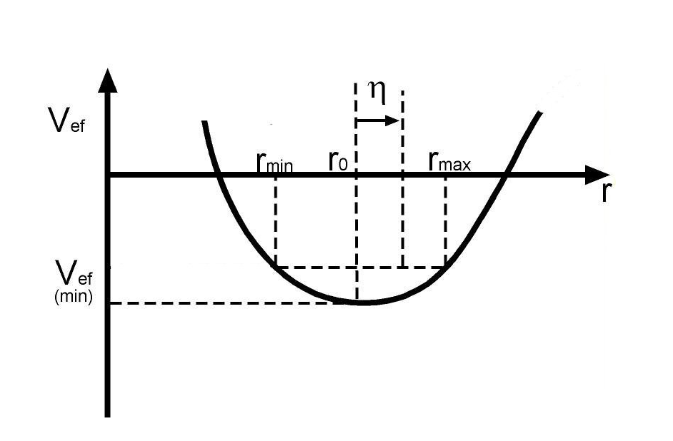
\includegraphics[width=2.0in]{Figuras/EstabilidadEta.png}
   	\end{figure}
	\item<3-> Desarrollamos por Taylor de la funci�n $V_{\mathrm{ef}}(r)$ alrededor de $r_0$, y tenemos
	$V_{\mathrm{ef}}(r)=V_{\mathrm{ef}}\left(r_0\right)+ \cancelto{0}{\left.\frac{\partial V_{\mathrm{ef}}}{\partial r}\right|_{r_0}}\left(r-r_0\right)+\left.\frac{1}{2} \frac{\partial^2 V_{\mathrm{ef}}}{\partial r^2}\right|_{r_0}\left(r-r_0\right)^2+\ldots$
	\item<4-> El primer t�rmino es una constante, $V_{\mathrm{ef}}\left(r_0\right)=$ cte, y puede ser suprimido  el segundo t�rmino se anula por ser un m�nimo.

    \end{itemize}
}
%%%%% Diapo 2
\section{Oscilaciones radiales}
\frame{
  \frametitle{Oscilaciones radiales}
   \begin{itemize}  
  	\item<1-> A segundo orden  $V_{\mathrm{ef}}(r)=\left.\frac{1}{2} \frac{\partial^2 V_{\mathrm{ef}}}{\partial r^2}\right|_{r_0}\left(r-r_0\right)^2+\ldots \approx \frac{1}{2} K \eta^2$, con $\left.K \equiv \frac{\partial^2 V_{\mathrm{ef}}}{\partial r^2}\right|_{r_0}=\mathrm{cte}$
	\item<2-> La ecuaci�n de movimiento radial, $\mu \ddot{r}=f_{\mathrm{ef}}(r)$ para $r=r_0+\eta$ resulta $\ddot{\eta}+\omega_r^2 \eta=0$
	\item<3-> Que la ecuaci�n de un oscilador arm�nico con frecuencia de oscilaci�n radial $\omega_r^2=\frac{K}{\mu}=\left.\frac{1}{\mu} \frac{\partial^2 V_{\mathrm{ef}}}{\partial r^2}\right|_{r_0}$
	 \begin{figure}[t]
		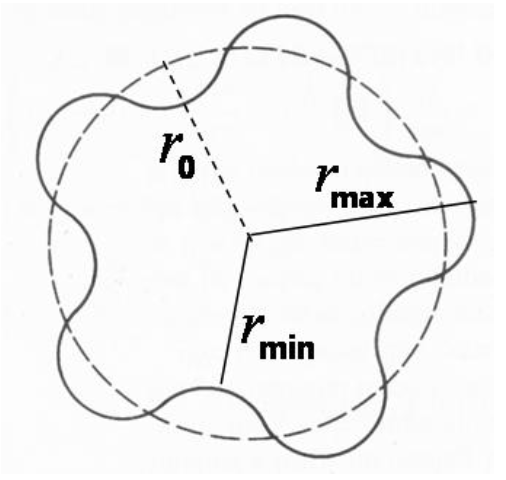
\includegraphics[width=1.5in]{Figuras/OscilaRadial.png}
   	\end{figure}
    \end{itemize}
}
%%%%% Diapo 2
\section{Estabilidad para $V(r)=\frac{-k}{r} e^{-(r / a)}$}
\frame{
  \frametitle{Estabilidad para $V(r)=\frac{-k}{r} e^{-(r / a)}$}
   \begin{itemize}  
  	\item<1-> Investigar la estabilidad de �rbitas circulares descritas por el potencial $V(r)=\frac{-k}{r} e^{-(r / a)}$ donde $k>0$ y $a>0$.
	\item<2->
    \end{itemize}
}

%%%%% Diapo 2
\section{Precesi�n}
\frame{
  \frametitle{Precesi�n}
   \begin{itemize}  
  	\item<1-> El �ngulo de precesi�n $\Delta \theta$ es el recorrido por la direcci�n del perihelio en el plano del movimiento durante un per�odo de oscilaci�n radial $T_r$. 
	\item<2-> Esto es $\Delta \theta=\dot{\theta} T_r=2 \pi \frac{\dot{\theta}}{\omega_r}$, y como  $\dot{\theta}=\frac{L}{\mu r_0^2}$, 
	\item<3-> tenemos $\Delta \theta=2 \pi \frac{L}{\mu r_0^2}\left(\left.\frac{1}{\mu} \frac{\partial^2 V_{\mathrm{ef}}}{\partial r^2}\right|_{r_0}\right)^{-1 / 2}$
	\item<4-> La direcci�n del perihelio $r_{\min }$ cambia en un �ngulo $\Delta \theta$ durante la precesi�n de la �rbita. 
	\item<5-> La condici�n para que ocurra precesi�n es que $\Delta \theta<2 \pi$; es decir, $\dot{\theta}<\omega_r$.
	 \begin{figure}[t]
		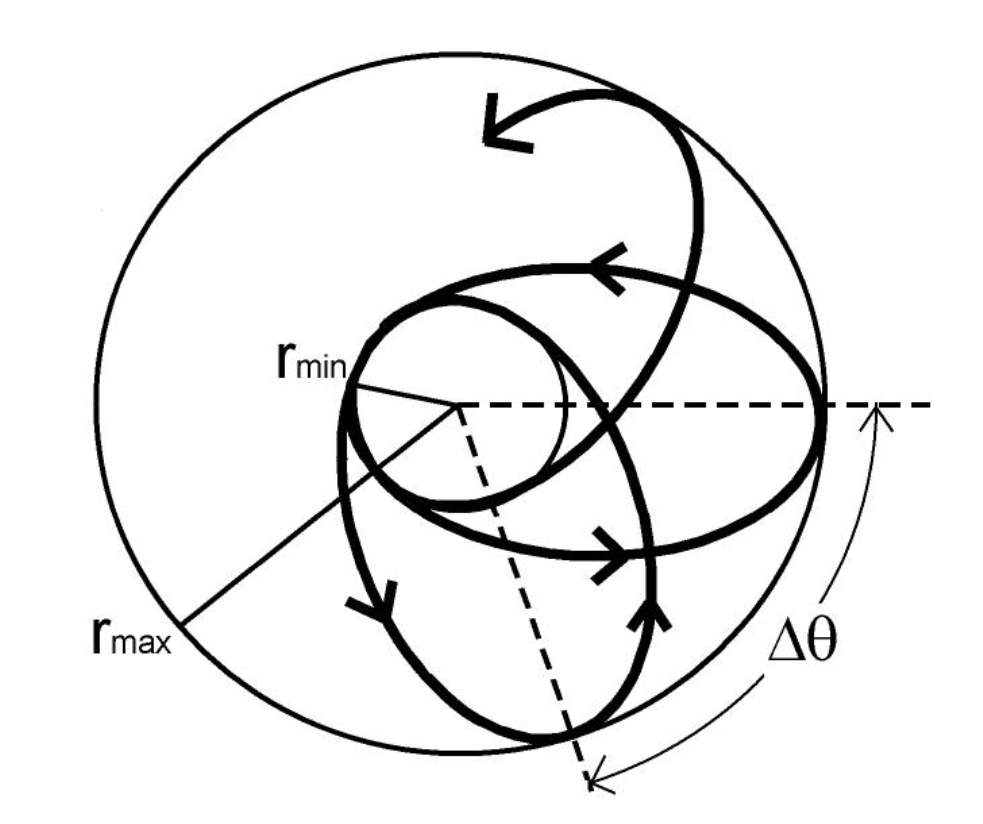
\includegraphics[width=1.5in]{Figuras/Precesa.png}
   	\end{figure}


    \end{itemize}
}
%
%%%%% Diapo 2
\section{Secci�n}
\frame{
  \frametitle{T�tulo transparencia}
   	\begin{itemize}  
  \item<1-> 
    \end{itemize}
}
%%%%% Diapo 2
\section{Secci�n}
\frame{
  \frametitle{T�tulo transparencia}
   	\begin{itemize}  
  \item<1-> 
    \end{itemize}
}
  
\end{document}
